\documentclass{amsart}
\usepackage[utf8]{inputenc}
\usepackage[russian]{babel}
\usepackage{gensymb}
\usepackage{MnSymbol}
\usepackage{graphicx}
\graphicspath{ {./img/} }

\begin{document}
Т7. Вписанный в окружность угол, стороны которого проходят через две данные точки окружности, равны половине угла между радиусами проведеными в эти точки, или дополняет половину этого угла до 180\degree

\textbf{Доказательство}

Надо доказать что $\angle AOC$ = 2 * $\angle ABC$   (1) \\*
Смотрите рисунок \\*

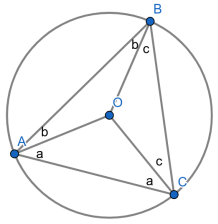
\includegraphics[scale=0.5]{vpisanii_v_okrujnosti}

Угол AOC можно записать как следующее равенство : \\*
$180-2a = 2[180-(a+b+a+c)]$  (2) \\*
$180-2a = 2(180-a-b-a-c)$ \\* 
$180-2a = 2(180-2a-b-c)$ \\*
$90-a = 180-2a-b-c$ \\*
$90 = 180-a-b-c$ \\*
$-180+90 = -a-b-c$ \\*
$-90 = -a-b-c$ \\*
$90 = a+b+c$ \\*

Угол ABC можно записать как равенство : \\*
$b+c = 180-(a+b+a+c)$ (3) \\*
$b+c = 180-a-b-a-c$ \\*
$-180 = -b-c-a-b-a-c$ \\*
$-180 = -2a-2b-2c$ \\*
$-90 = -a-b-c$ \\*
$90 = a+b+c$ \\*

Замечаем что равенства (2) и (3) идентичны

$\blacksquare$

\end{document}